\chapter{Work Completed}\label{C:work}

This chapter will discuss the work that has been completed so far on this project. It will begin by discussing the projects requirements', using them to design and justify the final specifications of the system. Once the specifications are outlined, the architecture and design of the final system will be discussed. Finally the design and current implementation of the PWM signal generator will be specified.  

\section{Defining \& Justifying System Specifications}\label{S:specs}

Based on the system requirements that have been outlined in \Cref{C:intro}, a set of system specifications can be created to inform the design. Current work on this project has been towards the implementation of the PWM signal generator, and as such all specifications outlined will pertain to this work.

The final system is required to be able to select both the output voltage and inductor current ripple of the buck converter. From this requirement we specify that our PWM generator must vary both the duty cycle and the switching frequency of the buck converter, based on \Cref{E:V_out} \& \Cref{E:delta_i}. The requirements also specify the level of precision that will be required for these selections, allowing us to specify the tolerable error. Using these same equations, the minimum duty cycle step size in \Cref{E:duty_step}, the inductor minimum and maximum values in \Cref{E:L_min} \& \Cref{E:L_max}, and the frequency step size in \Cref{E:f_step} have all been derived. For the derivation of these values see \Cref*{A:specs}.\\

Duty cycle step calculation:
\begin{align}
    V_{error} &= V_{min} \cdot error = 0.15V\\
    D_{step} &= \frac{V_{error}}{V_{in}} = 0.0125\\
    N_{step} &= \frac{1}{D_{step}} = 80 \label{E:duty_step}
\end{align}

Inductor Sizing Calculations:
\begin{align}
    L_{max}&=\frac{V_{max}\cdot\left(1-D_{max}\right)}{f_{min}\cdot I_{min}} = 27.7mH \label{E:L_max}\\ 
    L_{min}&=\frac{\frac{V_{in}}{2}\cdot\left(1-0.5\right)}{f_{max}\cdot I_{min}} = 0.5mH \label{E:L_min}
\end{align}

Frequency step calculation:
\begin{align}
    f_{step}&=\frac{V_{max}\cdot\left(1-D_{max}\right)}{\left(I_{min}-I_{Error}\right)\cdot L_{max}}-f_{min} = 52Hz\\
    N_{steps}&=\frac{\left(f_{max}-f_{min}\right)}{f_{step}} = 1881 \label{E:f_step}
\end{align}

From these equations we can build a list of final specifications to inform the design of our PWM generator and buck converter. The PWM generator must provide a minimum voltage step size of $0.0125V$, for a resolution of 80 voltage steps between 3V and 10V. The PWM generator must also be able to provide a minimum frequency step size of $52Hz$, for a resolution of 1881 frequency steps between $1KHz$ \& $100kHz$. Finally we can also specify that the buck converter must be capable of functioning with inductor values between $0.5mH$ \& $27.7mH$. \\

By designing the PWM generator and the buck converter to these specifications, we are able to guarantee that we can always achieve the requirements outlined in \Cref{C:intro}.

\section{System Architecture \& Design}\label{S:system}

To achieve the specifications that have been outlined in \Cref{S:specs}, it is important to design the system architecture around them. In \Cref{F:sys_overview} an overview of the system architecture can be seen, with three main design sections outlined. These sections each represent a significant segment of work that must be completed for the final artefact of this project to be achieved. \\

The first section of work that must be completed is the design of the PWM generation, denoted 1 in \Cref{F:sys_overview}. This PWM generator will be used to control both the output voltage and the inductor current ripple, and as such must be able to modulate both the duty cycle and the frequency of the PWM to the precisions required. \\

The second section of work is the design of the sensing elements required by the system, denoted 2 in \Cref{F:sys_overview}. These elements will be used to measure both the output voltage and the inductor current ripple, and therefor must be able to achieve the required precisions and sampling rates. \\

Finally the third section of work is the design and implementation of the two control systems, denoted 3 in \Cref{F:sys_overview}. These control systems will be responsible for maintaining the desired output voltage and inductor current ripple of the buck converter. This system will therefor be responsible for facilitating the final functionality of the project, combining sections 1 \& 2. \\

\begin{figure}[!h]
    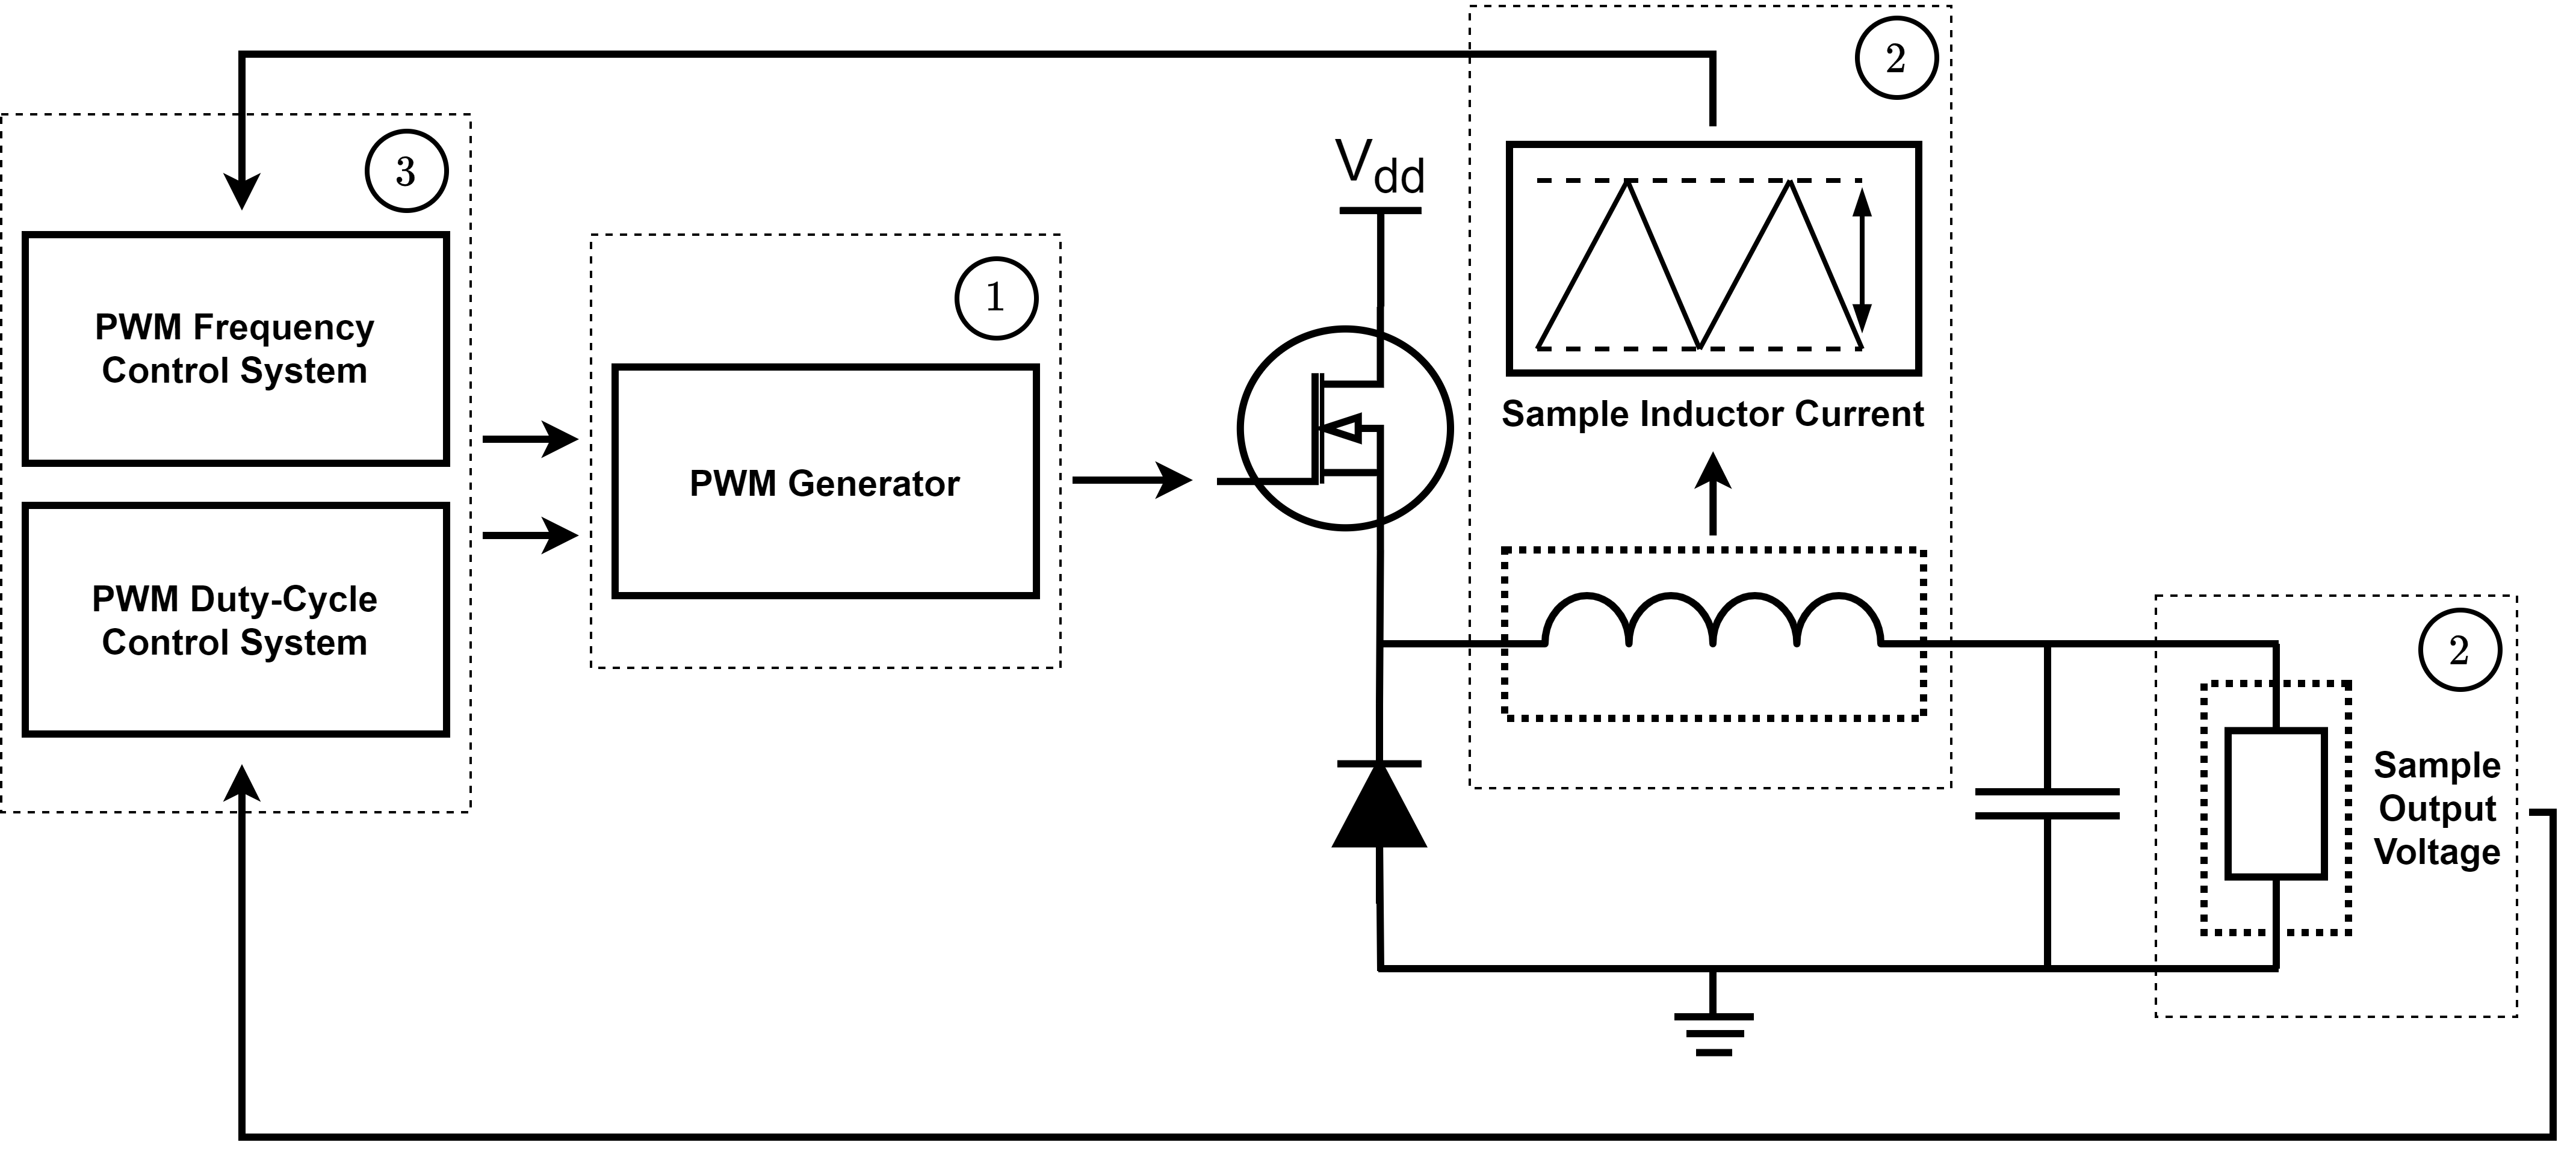
\includegraphics[width = 0.95\textwidth]{System_Overview.png}
    \caption{High level system overview}
    \vspace{-20pt}
    \label{F:sys_overview}
\end{figure}

\section{PWM Generation Design}\label{S:pwm_gen}

In the design of the PWM generator, both the analogue and digital designs discussed in \Cref{S:PWM} were considered, designed, and tested for. Each of these designs presented pros and cons that would affects the overall design of the system architecture. This section will discuss these designs and finalise the design of the PWM generator for this system. 

\subsection{Analogue PWM Generator Design}\label{S:analogue_design}

As discussed in \Cref{S:analogue_PWM}, the design of the analogue PWM signal generator requires three stages, each of which will have its own design requirements based on the specifications outlined in \Cref{S:specs}. \\

The clock generation stage will be responsible for setting the frequency of the final PWM signal. This specifies that the clock source have a variable frequency output range between $1kHz$ and $100kHz$, with a minimum step size of $52Hz$. Research was done on a variety of clock sources, looking at voltage-controlled oscillators (VCO's), signal generator IC's, and even the basic 555 timer. From this VCO's were identified to operate at much higher frequencies than those used in this project. It was also identified that signal generator IC's often require selections of passive components to operate effectively, increasing their complexity. For this reason the variable frequency 555 timer circuit was selected, as it provided the required specifications.\\

The next section designed was the signal integrator stage. This stage consisted of a basic op-amp integrator circuit, with a design requirement that it be able to integrate the clock signal across the frequency range required. This circuit was designed and implemented in an LTSpice simulation to evaluate it's performance, and can be seen in \Cref*{A:analogue_PWM}. From this simulation it was noted that the integrator's frequency response was similar to that of a first order low pass filter, and greatly attenuated the integrated signal. For this reason it was decided that analogue PWM generation would not be implemented in this system, as it presented many issues.

\subsection{Digital PWM Generator Design}\label{S:digital_design}

As discussed in \Cref{S:digital_PWM}, The design of the digital PWM generator is far simpler than that of the analogue, and can be implemented in a wide variety of methods. In this project microcontrollers and FPGA's have been considered.

Based solely on the capabilities of the platform, the PWM generator would be best designed and implemented on an FPGA as it would allow for superior speed and precision. However FGPA design brings a lot of difficulties, primarily in the prototyping and testing stages. Because of this, due to the limited time from of this project, we have decided to implement this PWM design using a microcontroller.

The selection of the microcontroller is highly dependant on the clock frequency and design of the PWM peripherals, as it must be capable of achieving the specifications outlined in \Cref{S:specs}. A large selection of microcontroller datasheets were reviewed to identify their specifications, including AVR, STM8, Espressif, and teensy based microcontrollers. From this review it was decided that the ESP32 microcontroller would be best suited to this project \cite{ESP32Manual}. This microcontroller is capable of outputting a maximum PWM frequency 125$kHz$ with a duty cycle resolution of 9 bits (512 voltage steps). From here a short C program was written to test the PWM functionality of the ESP32, and it was confirmed that it met the required specifications. The source code and images of this PWM signal can be found in \Cref{A:digital_PWM}.